\documentclass{article} % For LaTeX2e
% We will use NIPS submission format
\usepackage{graphicx}
\usepackage{epstopdf}
\usepackage{nips13submit_e,times}
% for hyperlinks
\usepackage{hyperref}
\usepackage{url}
% For figures
\usepackage{graphicx} 
\usepackage{subfigure} 
% math packages
\usepackage{amsmath}
\usepackage{amsfonts}
\usepackage{amsopn}
\usepackage{ifthen}
\usepackage{natbib}

\usepackage[utf8]{inputenc}
\usepackage[T1]{fontenc}
\usepackage{lmodern}


% tables
\usepackage{float}
\usepackage{booktabs}
\usepackage{multirow}
\usepackage{caption}

\title{Repeated Prisoner's Dilemma with Children}

\author{
Marco Goretti \\
\texttt{} \\
}


\nipsfinalcopy 


\begin{document}

\maketitle

\begin{abstract}
This paper studies the behaviour of children (between 7 and 15 years old) from schools near Lausanne (Switzerland) in the context of a prisoner's dilemma repeated over 3 rounds. The aspects analysed are the willfulness to continue cooperation depending on the previously played strategy as well as their capacity to reach the best utility for themselves and the group through cooperation.

Males in MM(Male - Male) groups were found to cooperate less than females in both FF (Female - Female) and mixed groups. The age of the player and the possibility to communicate significantly improved the willingness to cooperate.

To ability to communicate, the age and being a FF group instead of MM increased both the personal and total payoff.

A failure to cooperate greatly decreased the chances of reaching full cooperation in the next round while a betrayal (cooperation + defection) did not.


\end{abstract}

\section{Introduction}
Prisoner's dilemmas play a fundamental role in many microeconomic problems: they can help understand the behaviour of people in a wide range of situations that can go from simply continuing to work together to reaching the optimal allocation of resources for externalities.

The evolution in young children's behaviour is a topic that has been discussed in many psychological papers with a focus on the reason of the behaviour. This study will be more centred on the economic aspect of the matter, namely the behaviour itself and its implications on the personal and global utility.

The studied age goes from 8 to 15 years with most of the measures between 9 to 13. This age corresponds to preadolescence and the beginning of adolescence, which is after most changes in behaviour (more specifically development of inequality aversion and altruism) took place according to \cite{benen}, \cite{fehr} and \cite{fehr2}. \cite{kogut} discusses the evolution of inequity aversion in the following years and indicates a reinforcement of the previously mentioned behaviour.

Many papers find contrasting results on the topic of cooperation between groups of males, groups of females and mixed groups in adults. The meta-analysis made by \cite{balliet} finds that there is more cooperation in male-male interactions than in female-female interactions, while females cooperate more in mixed-sex interactions. A study done by \cite{card} on the difference of cooperation between children in two countries of very different socio-economical status, Colombia and Sweden, finds that in bad socioeconomic context females cooperate less than males while the opposite is found in children of good SES (socioeconomic status).

The vocation of this study is to compare the previously mentioned results to those observed with Swiss children in a context in which they all know each other beforehand and analyze those findings from the point of view of the standard theory on repeated prisoner's dilemmas and cooperation in general.


\section{Methodology}
The study was conducted at the university of Lausanne, during 2 school days, with kids from neighbouring schools of an age ranging from 7 to 15 years old. A second part of this study took place in the following week-end but this analysis will only talk about the school kids because their data is cleaner and less heterogeneous.
During this study, children from the same class formed groups of 2 and participated in a prisoner's dilemma repeated over 3 rounds: in every round each player had to choose between cooperating (Green card) or defecting (Red card). At the end of the game, they are rewarded with a number of candies equal to the sum of the payoffs of each round that is given as follows: 
\begin{table}[H]
\centering

\begin{tabular}{ r|c|c| }
\multicolumn{1}{r}{P1 \textbackslash P2}
 &  \multicolumn{1}{c}{Green}
 & \multicolumn{1}{c}{Red} \\
\cline{2-3}
Green & (3,3) & (0, 5) \\
\cline{2-3}
Red & (5,0) & (1,1) \\
\cline{2-3}
\end{tabular}

\end{table}

\textbf{Convention: In this paper the a posteriori result GG will be called cooperation, RR defection and RG or GR betrayal.}

Each round is a standard prisoner's dilemma resulting in the whole setup being a repeated prisoner's dilemma. 

Half of the participants were given the possibility to communicate while the others were not. The standard results regarding communication and the possibility of making promises say that cooperation should be more likely thus increasing the global utility.

The selfish persons' Nash equilibrium for the subproblem is RR giving by backward induction that RR is the best strategy for every round. In the case of strongly inequity averse (or tit for tat) players the best strategy will be to always play GG and finally for the mixed case of a selfish with a tit for tat they should play GG in the 2 first rounds and, finally, the selfish will play R. If there is an incertitude regarding the type of the other player (which should be mitigated by the fact that the players know each other) they should play the last enunciated strategy.

All regressions were done using a cluster on the group id to correct the standard error for the fact that there are 3 times more measures than actual users and that users in the same group are linked.
\section{Data Analysis}

\begin{table}[H]
\centering
\caption{\label{}\textbf{Players by age}}
\begin{tabular}{l|lll}
\hline
      & Sexe &        &       \\
Age   & Male & Female & Total \\ \hline
7     & 3    &        & 3     \\
8     & 9    & 14     & 23    \\
9     & 137  & 85     & 222   \\
10    & 249  & 238    & 487   \\
11    & 377  & 349    & 726   \\
12    & 250  & 265    & 515   \\
13    & 170  & 167    & 337   \\
14    & 26   & 43     & 69    \\
15    & 6    & 6      & 12    \\ \hline
Total & 1277 & 1167   & 2394  \\ \hline
\end{tabular}
\end{table}

This distribution of sex by age does not show any anomaly that could threaten external validity (the sampling is close to the general children population in Switzerland) besides the overrepresentation of 9 years old males which is still small.

\subsection{Behaviour}
Figure \ref{fig:round} shows that being able to communicate increases greatly (almost doubles) the chances that a player will play the green card (cooperation choice). 

Girls cooperate more often than boys but seem to cooperate less as the rounds advance in the case without communication.

In the case with communication, it can be seen that groups composed exclusively of girls cooperate better than others. All the groups except MM cooperate less during the second round.

\begin{figure}[H]
\centering
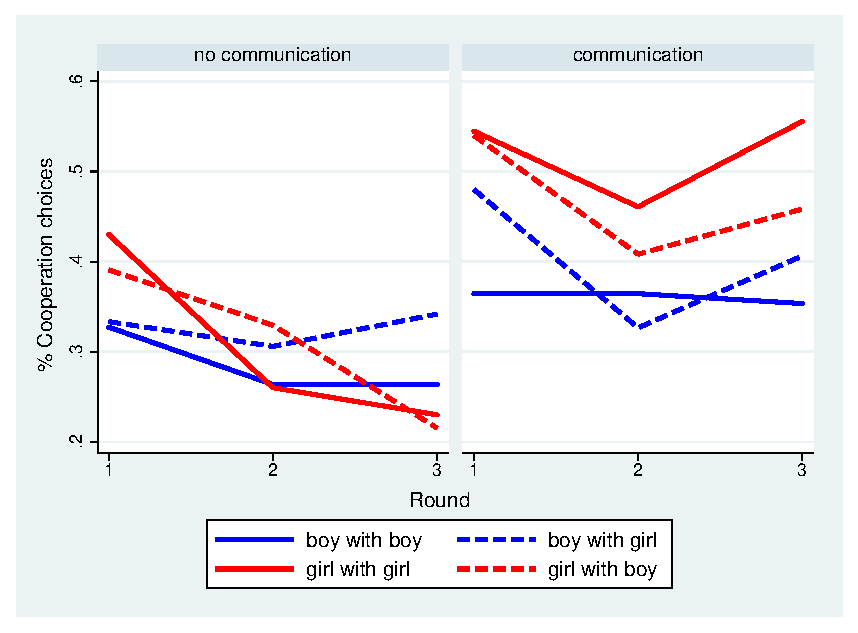
\includegraphics[scale=.7]{inc/round.eps}
\caption{Cooperation percentage by communication}
\label{fig:round}
\end{figure}

Figure \ref{fig:roundBar} shows the same kind of statistics as  \ref{fig:round} but instead of having a binary output it has 4 states which are the 4 possible results (cooperation, defection, 1 betrays 2 and 2 betrays 1). The difference in cooperation (GG) between MM and the other groups is easily seen. However, the only apparent difference in betrayal can be found in round 3 when comparing MM with FF (There are almost twice as many RG and GR played by MM than FF in round 3).

\begin{figure}[H]
\centering
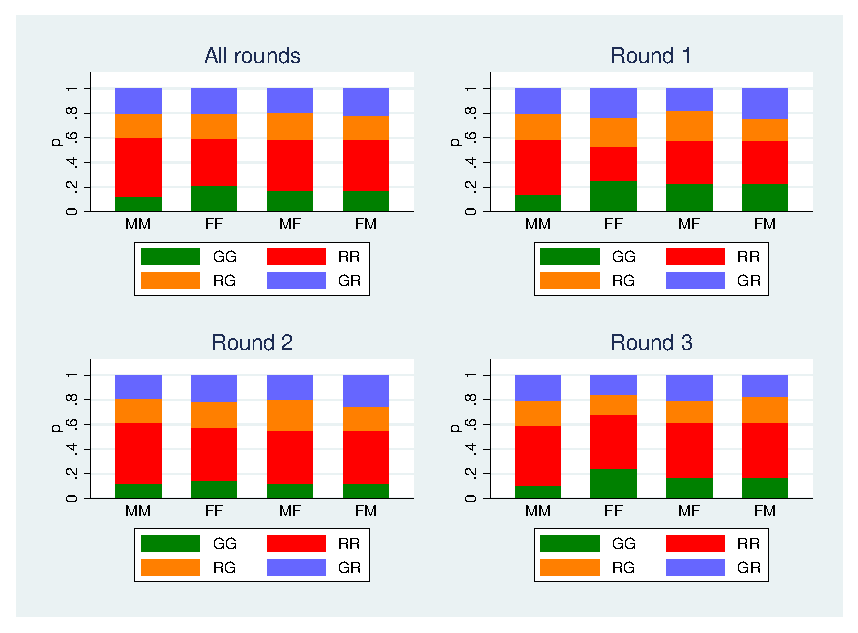
\includegraphics[scale=1]{inc/roundBar.eps}
\caption{Played strategies}
\label{fig:roundBar}
\end{figure}

\subsection{Total utility}
Figure \ref{fig:totalPayoff} shows that MM groups reach the lowest group payoff, FF the highest and, even though the mixed group is in between the others, the personal payoff of the male in the mixed group is higher than that of the female (he betrays her more often) giving him almost the same personal payoff as females in the FF group.
\begin{figure}[H]
\centering
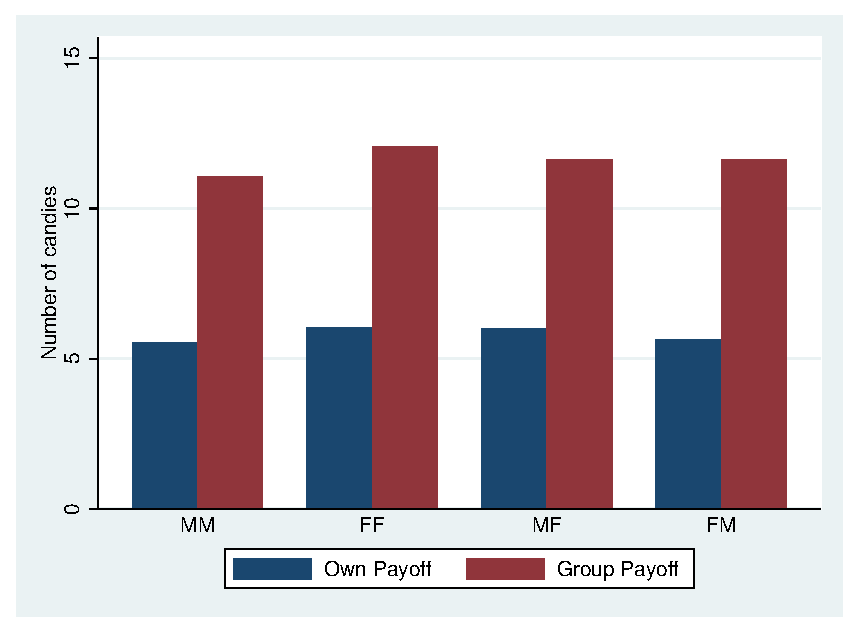
\includegraphics[scale=.7]{inc/totalPayoff.eps}
\caption{Payoff over the 3 rounds by group composition}
\label{fig:totalPayoff}
\end{figure}

A trend can be seen in Figure \ref{fig:age} where age correlates positively with both the personal and group payoff. At least for the first years or for the mixed and female groups.
\begin{figure}[H]
\centering
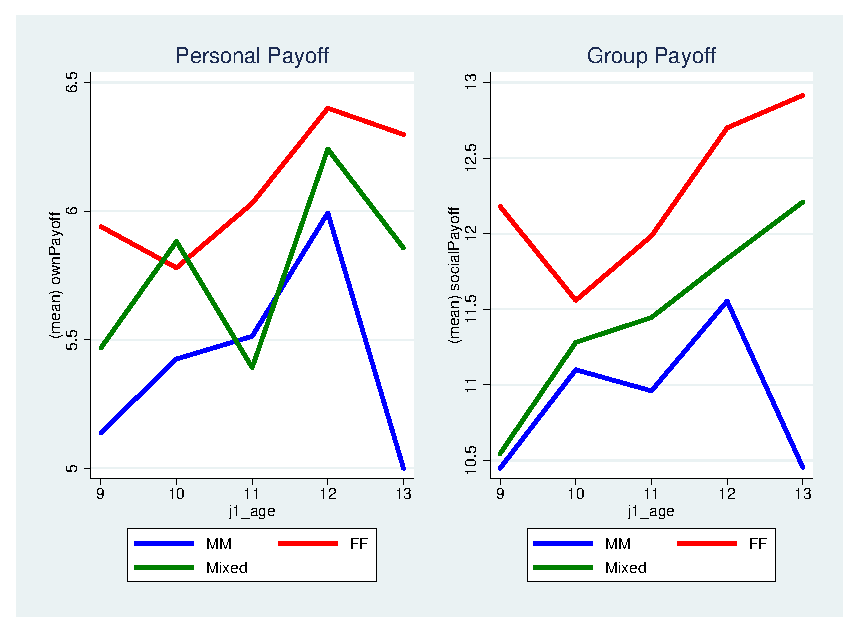
\includegraphics[scale=1]{inc/age.eps}
\caption{Payoff over the 3 rounds by age}
\label{fig:age}
\end{figure}

\section{Results}
Most of the regressions will be displayed as pairs; first a linear regression to show a linear approximation of the influence of the regressor and then the first order derivative of the logistic regression to find the exact value. Given that we want to estimate a probability and that there is no guarantee that the explained variable is homogeneously represented on each dimension we cannot affirm that OLS will give a non-biased estimation of the probability thus using a logistic regression, or any other sort of non-linear binary classification, is needed to have reliable p-values.
\subsection{Behaviour}
%behav_results
\begin{table}[H]
\caption{Probability that a kid collaborates} \label{tab:behav_results}

\begin{center}
\begin{tabular}{lcccc} \hline
 & (1) & (2) & (3) & (4) \\
Cooperation & p OLS & p OLS & p Logit & p Logit \\ \hline


\vspace{4pt} & \begin{footnotesize}\end{footnotesize} & \begin{footnotesize}\end{footnotesize} & \begin{footnotesize}\end{footnotesize} & \begin{footnotesize}\end{footnotesize} \\
Age & 0.023** & 0.023** & 0.023** & 0.023** \\
\vspace{4pt} & \begin{footnotesize}(0.009)\end{footnotesize} & \begin{footnotesize}(0.009)\end{footnotesize} & \begin{footnotesize}(0.009)\end{footnotesize} & \begin{footnotesize}(0.009)\end{footnotesize} \\
Communication & 0.130*** & 0.130*** & 0.132*** & 0.132*** \\
\vspace{4pt} & \begin{footnotesize}(0.023)\end{footnotesize} & \begin{footnotesize}(0.023)\end{footnotesize} & \begin{footnotesize}(0.024)\end{footnotesize} & \begin{footnotesize}(0.024)\end{footnotesize} \\
Age difference & -0.002 & -0.002 & -0.002 & -0.002 \\
\vspace{4pt} & \begin{footnotesize}(0.018)\end{footnotesize} & \begin{footnotesize}(0.018)\end{footnotesize} & \begin{footnotesize}(0.019)\end{footnotesize} & \begin{footnotesize}(0.019)\end{footnotesize} \\
Female & 0.061*** &  &  &  \\
\vspace{4pt} & \begin{footnotesize}(0.020)\end{footnotesize} & \begin{footnotesize}\end{footnotesize} & \begin{footnotesize}\end{footnotesize} & \begin{footnotesize}\end{footnotesize} \\
groupGender = 1, FF &  & 0.089*** & 0.091*** &  \\
\vspace{4pt} & \begin{footnotesize}\end{footnotesize} & \begin{footnotesize}(0.032)\end{footnotesize} & \begin{footnotesize}(0.032)\end{footnotesize} & \begin{footnotesize}\end{footnotesize} \\
groupGender = 2, MF &  & 0.039 & 0.039 & -0.052 \\
\vspace{4pt} & \begin{footnotesize}\end{footnotesize} & \begin{footnotesize}(0.031)\end{footnotesize} & \begin{footnotesize}(0.031)\end{footnotesize} & \begin{footnotesize}(0.033)\end{footnotesize} \\
groupGender = 3, FM &  & 0.066** & 0.067** & -0.024 \\
\vspace{4pt} & \begin{footnotesize}\end{footnotesize} & \begin{footnotesize}(0.029)\end{footnotesize} & \begin{footnotesize}(0.029)\end{footnotesize} & \begin{footnotesize}(0.031)\end{footnotesize} \\
groupGender = 0, MM &  &  &  & -0.091*** \\
\vspace{4pt} & \begin{footnotesize}\end{footnotesize} & \begin{footnotesize}\end{footnotesize} & \begin{footnotesize}\end{footnotesize} & \begin{footnotesize}(0.032)\end{footnotesize} \\
Constant & 0.019 & 0.005 &  &  \\
 & \begin{footnotesize}(0.102)\end{footnotesize} & \begin{footnotesize}(0.102)\end{footnotesize} & \begin{footnotesize}\end{footnotesize} & \begin{footnotesize}\end{footnotesize} \\
\vspace{4pt} & \begin{footnotesize}\end{footnotesize} & \begin{footnotesize}\end{footnotesize} & \begin{footnotesize}\end{footnotesize} & \begin{footnotesize}\end{footnotesize} \\
Observations & 2,394 & 2,394 & 2,394 & 2,394 \\
 $R^2$ & 0.027 & 0.028 &  &  \\ \hline\hline
 
\multicolumn{5}{c}{\begin{footnotesize} Clustered standard errors in parentheses\end{footnotesize}} \\
\multicolumn{5}{c}{\begin{footnotesize} *** p$<$0.01, ** p$<$0.05, * p$<$0.1\end{footnotesize}} \\
\end{tabular}
\end{center}


\end{table}

%text
Table \ref{tab:behav_results} presents the  probability of a player choosing to collaborate. The age and possibility to communicate with the other players have a significant effect on their willingness to participate ($+25\%$ between 13 year-old that can communicate and 8 year-old that cannot communicate).
Females have an overall probability 6\% higher than males which can be decomposed by the composition of the group (also taking the opponent's sex into account) showing that a group composed only of girls will have a 9\% higher probability than a group of males while also having a significant effect on the mixed group . From the male point of view, the effect of being in a mixed group instead of a male-only is not significant (the male will not cooperate more with a female, while a female will cooperate more with a male than males together).

The influence of the communication is in line with the standard results on the matter, while the higher cooperation of females in the full females group opposes the behaviour found in adults in Sex Differences in Cooperation. 

\vspace{1.5 cm}

Table \ref{tab:total_round} finds that the interaction between the round and the composition of the group when they can communicate described in Figure \ref{fig:round} is not significant (only marginally significant for MF).

The influence of age is only significant when the players can communicate.


%total_round
\begin{table}[H]
\caption{Interaction between gender and round on the probability that a kid collaborates } \label{tab:total_round}

\begin{center}
\begin{tabular}{lccc} \hline
 & (1) & (2) & (3) \\
Cooperation & total & No Coop & Coop \\ \hline
\vspace{4pt} & \begin{footnotesize}\end{footnotesize} & \begin{footnotesize}\end{footnotesize} & \begin{footnotesize}\end{footnotesize} \\
Age & 0.024** & 0.011 & 0.034*** \\
\vspace{4pt} & \begin{footnotesize}(0.010)\end{footnotesize} & \begin{footnotesize}(0.013)\end{footnotesize} & \begin{footnotesize}(0.013)\end{footnotesize} \\
groupGender==FF & 0.135*** & 0.091 & 0.175** \\
\vspace{4pt} & \begin{footnotesize}(0.048)\end{footnotesize} & \begin{footnotesize}(0.061)\end{footnotesize} & \begin{footnotesize}(0.071)\end{footnotesize} \\
groupGender==MF & 0.063 & 0.006 & 0.110 \\
\vspace{4pt} & \begin{footnotesize}(0.049)\end{footnotesize} & \begin{footnotesize}(0.065)\end{footnotesize} & \begin{footnotesize}(0.071)\end{footnotesize} \\
groupGender==FM & 0.117** & 0.057 & 0.168** \\
\vspace{4pt} & \begin{footnotesize}(0.049)\end{footnotesize} & \begin{footnotesize}(0.064)\end{footnotesize} & \begin{footnotesize}(0.072)\end{footnotesize} \\
round==2 & -0.033 & -0.065 & 0.000 \\
\vspace{4pt} & \begin{footnotesize}(0.046)\end{footnotesize} & \begin{footnotesize}(0.063)\end{footnotesize} & \begin{footnotesize}(0.066)\end{footnotesize} \\
round==3 & -0.039 & -0.065 & -0.011 \\
\vspace{4pt} & \begin{footnotesize}(0.044)\end{footnotesize} & \begin{footnotesize}(0.070)\end{footnotesize} & \begin{footnotesize}(0.051)\end{footnotesize} \\
groupGender==FF, round==2 & -0.092 & -0.097 & -0.081 \\
\vspace{4pt} & \begin{footnotesize}(0.064)\end{footnotesize} & \begin{footnotesize}(0.090)\end{footnotesize} & \begin{footnotesize}(0.091)\end{footnotesize} \\
groupGender==FF, round==3 & -0.048 & -0.131 & 0.022 \\
\vspace{4pt} & \begin{footnotesize}(0.062)\end{footnotesize} & \begin{footnotesize}(0.094)\end{footnotesize} & \begin{footnotesize}(0.083)\end{footnotesize} \\
groupGender==MF, round==2 & -0.065 & 0.038 & -0.162* \\
\vspace{4pt} & \begin{footnotesize}(0.065)\end{footnotesize} & \begin{footnotesize}(0.087)\end{footnotesize} & \begin{footnotesize}(0.094)\end{footnotesize} \\
groupGender==MF, round==3 & 0.005 & 0.073 & -0.064 \\
\vspace{4pt} & \begin{footnotesize}(0.067)\end{footnotesize} & \begin{footnotesize}(0.099)\end{footnotesize} & \begin{footnotesize}(0.088)\end{footnotesize} \\
groupGender==FM, round==2 & -0.064 & 0.008 & -0.134 \\
\vspace{4pt} & \begin{footnotesize}(0.071)\end{footnotesize} & \begin{footnotesize}(0.095)\end{footnotesize} & \begin{footnotesize}(0.102)\end{footnotesize} \\
groupGender==FM, round==3 & -0.081 & -0.114 & -0.072 \\
 & \begin{footnotesize}(0.067)\end{footnotesize} & \begin{footnotesize}(0.100)\end{footnotesize} & \begin{footnotesize}(0.090)\end{footnotesize} \\
\vspace{4pt} & \begin{footnotesize}\end{footnotesize} & \begin{footnotesize}\end{footnotesize} & \begin{footnotesize}\end{footnotesize} \\
 Observations & 2,394 & 1,132 & 1,262 \\ \hline
\multicolumn{4}{c}{\begin{footnotesize} Clustered standard errors in parentheses\end{footnotesize}} \\
\multicolumn{4}{c}{\begin{footnotesize} *** p$<$0.01, ** p$<$0.05, * p$<$0.1\end{footnotesize}} \\
\end{tabular}
\end{center}

\end{table}



\subsection{Total utility}
%total_results

\begin{table}[H]
\caption{Payoff over the 3 rounds} \label{tab:total_results}

\begin{center}
\begin{tabular}{lcccc} \hline
 & (1) & (2) & (3) & (4) \\
Payoff & Own & Own & Group & Group \\ \hline
\vspace{4pt} & \begin{footnotesize}\end{footnotesize} & \begin{footnotesize}\end{footnotesize} & \begin{footnotesize}\end{footnotesize} & \begin{footnotesize}\end{footnotesize} \\
Group age & 0.129* & 0.129* & 0.258* & 0.258* \\
\vspace{4pt} & \begin{footnotesize}(0.066)\end{footnotesize} & \begin{footnotesize}(0.066)\end{footnotesize} & \begin{footnotesize}(0.132)\end{footnotesize} & \begin{footnotesize}(0.132)\end{footnotesize} \\
Communication & 0.786*** & 0.786*** & 1.573*** & 1.573*** \\
\vspace{4pt} & \begin{footnotesize}(0.161)\end{footnotesize} & \begin{footnotesize}(0.161)\end{footnotesize} & \begin{footnotesize}(0.322)\end{footnotesize} & \begin{footnotesize}(0.322)\end{footnotesize} \\
Age difference & -0.039 & -0.039 & -0.078 & -0.078 \\
\vspace{4pt} & \begin{footnotesize}(0.122)\end{footnotesize} & \begin{footnotesize}(0.122)\end{footnotesize} & \begin{footnotesize}(0.243)\end{footnotesize} & \begin{footnotesize}(0.243)\end{footnotesize} \\
groupGender = 1, FF & 0.481** &  & 0.961** &  \\
\vspace{4pt} & \begin{footnotesize}(0.217)\end{footnotesize} & \begin{footnotesize}\end{footnotesize} & \begin{footnotesize}(0.435)\end{footnotesize} & \begin{footnotesize}\end{footnotesize} \\
groupGender = 2, MF & 0.443* & -0.038 & 0.491 & -0.470 \\
\vspace{4pt} & \begin{footnotesize}(0.236)\end{footnotesize} & \begin{footnotesize}(0.238)\end{footnotesize} & \begin{footnotesize}(0.390)\end{footnotesize} & \begin{footnotesize}(0.392)\end{footnotesize} \\
groupGender = 3, FM & 0.048 & -0.432* & 0.491 & -0.470 \\
\vspace{4pt} & \begin{footnotesize}(0.260)\end{footnotesize} & \begin{footnotesize}(0.260)\end{footnotesize} & \begin{footnotesize}(0.390)\end{footnotesize} & \begin{footnotesize}(0.392)\end{footnotesize} \\
groupGender = 0, MM &  & -0.481** &  & -0.961** \\
\vspace{4pt} & \begin{footnotesize}\end{footnotesize} & \begin{footnotesize}(0.217)\end{footnotesize} & \begin{footnotesize}\end{footnotesize} & \begin{footnotesize}(0.435)\end{footnotesize} \\
Constant & 3.721*** & 4.202*** & 7.443*** & 8.404*** \\
 & \begin{footnotesize}(0.743)\end{footnotesize} & \begin{footnotesize}(0.754)\end{footnotesize} & \begin{footnotesize}(1.487)\end{footnotesize} & \begin{footnotesize}(1.508)\end{footnotesize} \\
\vspace{4pt} & \begin{footnotesize}\end{footnotesize} & \begin{footnotesize}\end{footnotesize} & \begin{footnotesize}\end{footnotesize} & \begin{footnotesize}\end{footnotesize} \\
Observations & 2,394 & 2,394 & 2,394 & 2,394 \\
 $R^2$ & 0.031 & 0.031 & 0.076 & 0.076 \\ \hline
\multicolumn{5}{c}{\begin{footnotesize} Clustered standard errors in parentheses\end{footnotesize}} \\
\multicolumn{5}{c}{\begin{footnotesize} *** p$<$0.01, ** p$<$0.05, * p$<$0.1\end{footnotesize}} \\
\end{tabular}
\end{center}

\end{table}

%text
As observed in the previous section, being able to communicate increases the probability of a player deciding to collaborate so this observation is the natural extension. 

The mean age of the group is only marginally significant. 

The effect of the composition of the group indicates that the FF composition reaches a higher payoff than MM but nothing can be said about the mixed groups.

\subsection{Reaction and Cooperation}
In this section, only the complete cooperation (Green Green) and defection (Red Red) are studied because the mixed results can come from several different reasons (special strategy, idiosyncratic behaviour, vengeance...) and separating those effects would be very hard without bringing any useful information for the scope of the paper.
\subsubsection{First round (no history) }

%first_coop
\begin{table}[H]
\caption{Game result in the first round} \label{tab:first_coop}

\begin{center}
\begin{tabular}{lcccc} \hline
 & (1) & (2) & (3) & (4) \\
Result & GG OLS & GG Logit & RR OLS & RR Logit\\ \hline


\vspace{4pt} & \begin{footnotesize}\end{footnotesize} & \begin{footnotesize}\end{footnotesize} & \begin{footnotesize}\end{footnotesize} & \begin{footnotesize}\end{footnotesize} \\
Group age & 0.008 & 0.008 & -0.038** & -0.040** \\
\vspace{4pt} & \begin{footnotesize}(0.017)\end{footnotesize} & \begin{footnotesize}(0.016)\end{footnotesize} & \begin{footnotesize}(0.018)\end{footnotesize} & \begin{footnotesize}(0.019)\end{footnotesize} \\
Communication & 0.147*** & 0.149*** & -0.071 & -0.073 \\
\vspace{4pt} & \begin{footnotesize}(0.039)\end{footnotesize} & \begin{footnotesize}(0.041)\end{footnotesize} & \begin{footnotesize}(0.047)\end{footnotesize} & \begin{footnotesize}(0.048)\end{footnotesize} \\
Age difference & -0.023 & -0.023 & -0.018 & -0.019 \\
\vspace{4pt} & \begin{footnotesize}(0.027)\end{footnotesize} & \begin{footnotesize}(0.028)\end{footnotesize} & \begin{footnotesize}(0.037)\end{footnotesize} & \begin{footnotesize}(0.038)\end{footnotesize} \\
groupGender = 1, FF & 0.120** & 0.121** & -0.171*** & -0.173*** \\
\vspace{4pt} & \begin{footnotesize}(0.054)\end{footnotesize} & \begin{footnotesize}(0.054)\end{footnotesize} & \begin{footnotesize}(0.064)\end{footnotesize} & \begin{footnotesize}(0.064)\end{footnotesize} \\
groupGender = 2, MF & 0.086* & 0.086* & -0.087 & -0.088 \\
\vspace{4pt} & \begin{footnotesize}(0.045)\end{footnotesize} & \begin{footnotesize}(0.044)\end{footnotesize} & \begin{footnotesize}(0.059)\end{footnotesize} & \begin{footnotesize}(0.060)\end{footnotesize} \\
groupGender = 3, FM & 0.086* & 0.086* & -0.087 & -0.088 \\
\vspace{4pt} & \begin{footnotesize}(0.045)\end{footnotesize} & \begin{footnotesize}(0.044)\end{footnotesize} & \begin{footnotesize}(0.059)\end{footnotesize} & \begin{footnotesize}(0.060)\end{footnotesize} \\
Constant & -0.015 &  & 0.916*** &  \\
 & \begin{footnotesize}(0.188)\end{footnotesize} & \begin{footnotesize}\end{footnotesize} & \begin{footnotesize}(0.204)\end{footnotesize} & \begin{footnotesize}\end{footnotesize} \\
\vspace{4pt} & \begin{footnotesize}\end{footnotesize} & \begin{footnotesize}\end{footnotesize} & \begin{footnotesize}\end{footnotesize} & \begin{footnotesize}\end{footnotesize} \\
Observations & 826 & 826 & 826 & 826 \\
 $R^2$ & 0.048 &  & 0.036 &  \\ \hline

\multicolumn{5}{c}{\begin{footnotesize} Clustered standard errors in parentheses\end{footnotesize}} \\
\multicolumn{5}{c}{\begin{footnotesize} *** p$<$0.01, ** p$<$0.05, * p$<$0.1\end{footnotesize}} \\
\end{tabular}
\end{center}


\end{table}

%text

Table \ref{tab:first_coop} shows that communicating has a really strong effect on GG ($+15\%$) while having a non-significant effect on RR.

One interesting result is that every other group combination has a significantly higher chance of playing GG than the MM group meaning that MM obtain the worst a priori result.

Age only has a significant effect on reducing the chances of reaching the full defection situation ($-15\%$ from 8 to 12 years old) probably meaning that older kids understand better the negative consequences of starting with defection (they fear their opponent's reaction) and play green more often as it can be seen in the following table:
\begin{table}[htbp]\centering
\caption{\label{} 
\textbf{} }\begin{tabular} {@{} c c c @{}} \\ \hline
\textbf{Age} & \textbf{green percentage} &  \textbf{N}\\
\hline
       7  &          1 &          1 \\
       8  &   .5555556 &          9 \\
       9  &   .4078947 &         76 \\
      10  &   .3846154 &        169 \\
      11  &   .4244898 &        245 \\
      12  &   .4104046 &        173 \\
      13  &   .4869565 &        115 \\
      14  &       .625 &         24 \\
      15  &         .5 &          4 \\
   Total  &   .4289216 &        816 \\

\hline
\end{tabular}
\end{table}


\subsubsection{Other rounds (reaction) }
%last_coop
\begin{table}[H]
\caption{Game result in the second and last round} \label{tab:last_coop}

\begin{center}
\begin{tabular}{lccccc} \hline
 & (1) & (2) & (3) & (4) & (5) \\
Result & GG OLS& GG Logit & GG Logit& RR OLS& RR Logit\\ \hline

\vspace{4pt} & \begin{footnotesize}\end{footnotesize} & \begin{footnotesize}\end{footnotesize} & \begin{footnotesize}\end{footnotesize} & \begin{footnotesize}\end{footnotesize} & \begin{footnotesize}\end{footnotesize} \\
previousStrat = 2, Red Red & -0.130*** & -0.122** & -0.095* & 0.202*** & 0.210*** \\
\vspace{4pt} & \begin{footnotesize}(0.050)\end{footnotesize} & \begin{footnotesize}(0.047)\end{footnotesize} & \begin{footnotesize}(0.052)\end{footnotesize} & \begin{footnotesize}(0.053)\end{footnotesize} & \begin{footnotesize}(0.055)\end{footnotesize} \\
previousStrat = 3, Red Green & -0.080 & -0.074 & -0.047 & 0.068 & 0.072 \\
\vspace{4pt} & \begin{footnotesize}(0.050)\end{footnotesize} & \begin{footnotesize}(0.047)\end{footnotesize} & \begin{footnotesize}(0.050)\end{footnotesize} & \begin{footnotesize}(0.052)\end{footnotesize} & \begin{footnotesize}(0.054)\end{footnotesize} \\
previousStrat = 4, Green Red & -0.080 & -0.074 & -0.047 & 0.068 & 0.072 \\
\vspace{4pt} & \begin{footnotesize}(0.050)\end{footnotesize} & \begin{footnotesize}(0.047)\end{footnotesize} & \begin{footnotesize}(0.050)\end{footnotesize} & \begin{footnotesize}(0.052)\end{footnotesize} & \begin{footnotesize}(0.054)\end{footnotesize} \\
Group age & 0.035*** & 0.032*** & 0.032*** & -0.010 & -0.011 \\
\vspace{4pt} & \begin{footnotesize}(0.010)\end{footnotesize} & \begin{footnotesize}(0.009)\end{footnotesize} & \begin{footnotesize}(0.009)\end{footnotesize} & \begin{footnotesize}(0.014)\end{footnotesize} & \begin{footnotesize}(0.015)\end{footnotesize} \\
Age difference & 0.017 & 0.018 & 0.018 & 0.018 & 0.020 \\
\vspace{4pt} & \begin{footnotesize}(0.019)\end{footnotesize} & \begin{footnotesize}(0.018)\end{footnotesize} & \begin{footnotesize}(0.018)\end{footnotesize} & \begin{footnotesize}(0.026)\end{footnotesize} & \begin{footnotesize}(0.027)\end{footnotesize} \\
Communication & 0.077*** & 0.074*** & 0.075*** & -0.164*** & -0.171*** \\
\vspace{4pt} & \begin{footnotesize}(0.024)\end{footnotesize} & \begin{footnotesize}(0.024)\end{footnotesize} & \begin{footnotesize}(0.024)\end{footnotesize} & \begin{footnotesize}(0.036)\end{footnotesize} & \begin{footnotesize}(0.037)\end{footnotesize} \\
round = 3 & 0.048* & 0.046* & 0.035 & -0.004 & -0.004 \\
\vspace{4pt} & \begin{footnotesize}(0.025)\end{footnotesize} & \begin{footnotesize}(0.024)\end{footnotesize} & \begin{footnotesize}(0.028)\end{footnotesize} & \begin{footnotesize}(0.035)\end{footnotesize} & \begin{footnotesize}(0.037)\end{footnotesize} \\
GG * round == 3 &  &  & 0.042 &  &  \\
\vspace{4pt} & \begin{footnotesize}\end{footnotesize} & \begin{footnotesize}\end{footnotesize} & \begin{footnotesize}(0.037)\end{footnotesize} & \begin{footnotesize}\end{footnotesize} & \begin{footnotesize}\end{footnotesize} \\
groupGender = 1, FF & 0.057* & 0.055* & 0.057* & -0.027 & -0.028 \\
\vspace{4pt} & \begin{footnotesize}(0.035)\end{footnotesize} & \begin{footnotesize}(0.033)\end{footnotesize} & \begin{footnotesize}(0.033)\end{footnotesize} & \begin{footnotesize}(0.046)\end{footnotesize} & \begin{footnotesize}(0.049)\end{footnotesize} \\
groupGender = 2, MF & 0.013 & 0.014 & 0.015 & -0.031 & -0.033 \\
\vspace{4pt} & \begin{footnotesize}(0.028)\end{footnotesize} & \begin{footnotesize}(0.027)\end{footnotesize} & \begin{footnotesize}(0.026)\end{footnotesize} & \begin{footnotesize}(0.043)\end{footnotesize} & \begin{footnotesize}(0.045)\end{footnotesize} \\
groupGender = 3, FM & 0.013 & 0.014 & 0.015 & -0.031 & -0.033 \\
\vspace{4pt} & \begin{footnotesize}(0.028)\end{footnotesize} & \begin{footnotesize}(0.027)\end{footnotesize} & \begin{footnotesize}(0.026)\end{footnotesize} & \begin{footnotesize}(0.043)\end{footnotesize} & \begin{footnotesize}(0.045)\end{footnotesize} \\
Constant & -0.253** &  &  & 0.556*** &  \\
 & \begin{footnotesize}(0.109)\end{footnotesize} & \begin{footnotesize}\end{footnotesize} & \begin{footnotesize}\end{footnotesize} & \begin{footnotesize}(0.168)\end{footnotesize} & \begin{footnotesize}\end{footnotesize} \\
\vspace{4pt} & \begin{footnotesize}\end{footnotesize} & \begin{footnotesize}\end{footnotesize} & \begin{footnotesize}\end{footnotesize} & \begin{footnotesize}\end{footnotesize} & \begin{footnotesize}\end{footnotesize} \\
Observations & 1,568 & 1,568 & 1,568 & 1,568 & 1,568 \\
 $R^2$ & 0.059 &  &  & 0.063 &  \\ \hline
 
\multicolumn{6}{c}{\begin{footnotesize} Clustered standard errors in parentheses\end{footnotesize}} \\
\multicolumn{6}{c}{\begin{footnotesize} *** p$<$0.01, ** p$<$0.05, * p$<$0.1\end{footnotesize}} \\
\end{tabular}
\end{center}





\end{table}

%text
The only previous result providing a significant difference compared to GG is RR (the mixed strategies are marginally significant for the probability of GG but not RR).

Interestingly, the effect of age here is the opposite of what is observed in the first round: age significantly increases the probability of reaching GG but does not reduce the probability of playing RR. 

The effect of the gender of the group is more mitigated and the only marginally significant result is that FF have 5\% more chances of playing GG than MM.
A very interesting result that contrasts with the standard repeated game model is that there is a marginally significant higher probability of reaching GG in round 3 while the Nash equilibrium for this game is RR. The interaction between having played GG and being in round 3 is not significant so we cannot explain this effect by only saying that the players want to reward their opponent for having cooperated in the previous round. This means that there has to be another mechanic at play.

\section{Discussion}
\subsection{Summary of Findings}
Females were found to be more cooperative than males, both in female female groups and in mixed groups. However the payoff over the 3 rounds is only significantly different with a FF group compared to a MM group. Age only increases the probability of cooperating when the players can communicate, indicating an improvement of that communication.

The possibility to communicate significantly increases both the total payoff of the player and that of the group, showing an improved efficiency, while the mean age is only marginally significant. The difference in age was never found to be significant but it should also be considered that the children are in the same class, which means that there should never be a big gap in maturity level that could have a significant effect (but is not tested in this study since all the participants are from the same class). 

In the first round, male groups were found to play the Pareto optimum less often (respectively $-8.6\%$ and $-12\%$) than mixed or female groups, while age did not play any role. Communicating is still a major factor ($+15\%$).
Male groups have a $17\%$ higher probability of playing the worst case scenario (RR) than female groups but there is no significant difference between MM and the mixed groups. In the RR case, the age plays an important effect ($19\%$ for a 5 years difference) but communicating is not significant.

In the second and final round, the previously played strategy plays an important role: having previously played RR reduces the chances of playing GG by $13\%$ and increases those of playing RR by $20\%$, thus showing that there is not a strong will to resume cooperation after defection. Interestingly, a betrayal does only marginally reduce the probability of playing GG without increasing the chances of playing RR, which is what the standard theory would predict (always defection for selfish players or cooperation until betrayal and then total defection until the end in the presence of tit-for-tat players).

The age affects the opposite phenomenon than in the first round: it only increases the chances of playing GG. 

Communicating is still really useful as it increases the probability of playing GG by $7.7\%$ and decreases that of playing RR by $16.4\%$.

The gender of the group is less significant and only really plays a role for GG in the female group when compared to the male group and, even in that case, it is $5.7\%$, which is half of what was found for the first round.

Being in the last round increases the chances of playing GG. This effect is only partially explained by an interaction with the previously played strategy (reward for having cooperated before) since that interaction is not significant, but adding that effect makes the effect of being in round 3 non-significant.

%\subsection{Implications}
%Given the very specific context of the study, children from the same class thus knowing each other and a low payoff, there is no reason to suggest a broad validity of the findings. But even in the specific context those results can be applied for example to group composition at school where working on projects is similar to a prisoner's dilemma.

\subsection{Conclusion}
%The results obtained in this study finding that groups of women collaborate better than groups of men contradict several paper on the subject on adults (\cite{balliet}) but also on children of good SES (\cite{card}) which is the same context as this experiment. 

The results obtained in this study, namely that groups of women collaborate better than groups of men, contradict what is found in adults (\cite{balliet}) but is in line with some of the findings on children of good SES (\cite{card}): both this study and the paper find that girls collaborate better but they differ in the fact that the paper finds that girls collaborate better with boys than with other girls, while it is found here that they collaborate better together. 


The influence of age on cooperation does not contradict the implications of better collaboration given by the increased altruism \cite{kogut} and \cite{benen} for the younger children (7 - 10).  This study does not specifically test that effect and the continuous influence of age even after the age range of the previously quoted studies does not imply an extension of that result: kids could just get better with age at understanding what they have to do to improve their utility and communicate better as it can be seen in Table \ref{tab:total_round}.

The increased probability of cooperating in the last round seems to indicate a behaviour that is not described by the standard personalities (selfish, inequity averse or tit for tat).

%Another interesting study would have been to check the interaction between age and communication but the interaction effect in the regression was not significant while removing significance of age and communication

\bibliographystyle{plainnat}

\bibliography{bib}

\end{document}
